%\documentclass[20pt,margin=1in,innermargin=-4.5in,blockverticalspace=-0.25in]{tikzposter}
\documentclass[a1paper, landscape]{tikzposter}
%\geometry{paperwidth=42in,paperheight=32.5in}
\usepackage[utf8]{inputenc}
\usepackage{amsmath}
\usepackage{amsfonts}
\usepackage{amsthm}
\usepackage{amssymb}
\usepackage{mathrsfs}
\usepackage{graphicx}
\graphicspath{ {./images/} }
\usepackage{adjustbox}
\usepackage{enumitem}
\usepackage[backend=biber,style=numeric]{biblatex}
\usepackage{rutheme}
\usepackage{lipsum}
\usepackage{cancel}

\usepackage{mwe} % for placeholder images

\addbibresource{refs.bib}

% set theme parameters
\tikzposterlatexaffectionproofoff
\usetheme{RUTheme}
\usecolorstyle{RUStyle}

\usepackage[scaled]{helvet}
\renewcommand\familydefault{\sfdefault} 
\usepackage[T1]{fontenc}
\usepackage{hyperref}


\title{RU \LaTeX Poster Template}
\author{Author}
\institute{Reykjavík University}
\titlegraphic{
\includegraphics[width=0.1\textwidth]{ru_logo_transparent.png}}

% begin document
\begin{document}
\maketitle
\centering
\begin{columns}
    \column{0.32}
    \block{Info}{
        This is a poster template using the \texttt{tikzposter} package.
        It is based on Overleaf's poster template from UW-Madison, but with RU colors and font.
        The plotter uses A1 paper, so this template uses A1 paper.
    }
    \block{Hypothesis}
    {
         If~~$\displaystyle\lim_{x\rightarrow8}\frac{1}{x{-}8}=\infty$
~~then~~$\displaystyle\lim_{x\rightarrow5}\frac{1}{x{-}5}=\rotatebox{90}{5}$
    }
    \block{Proof}
    {
        \lipsum[2] \qed
    }

    \column{0.36}
    \block{Puffins}
    {
        \begin{tikzfigure}[Some puffins.]
            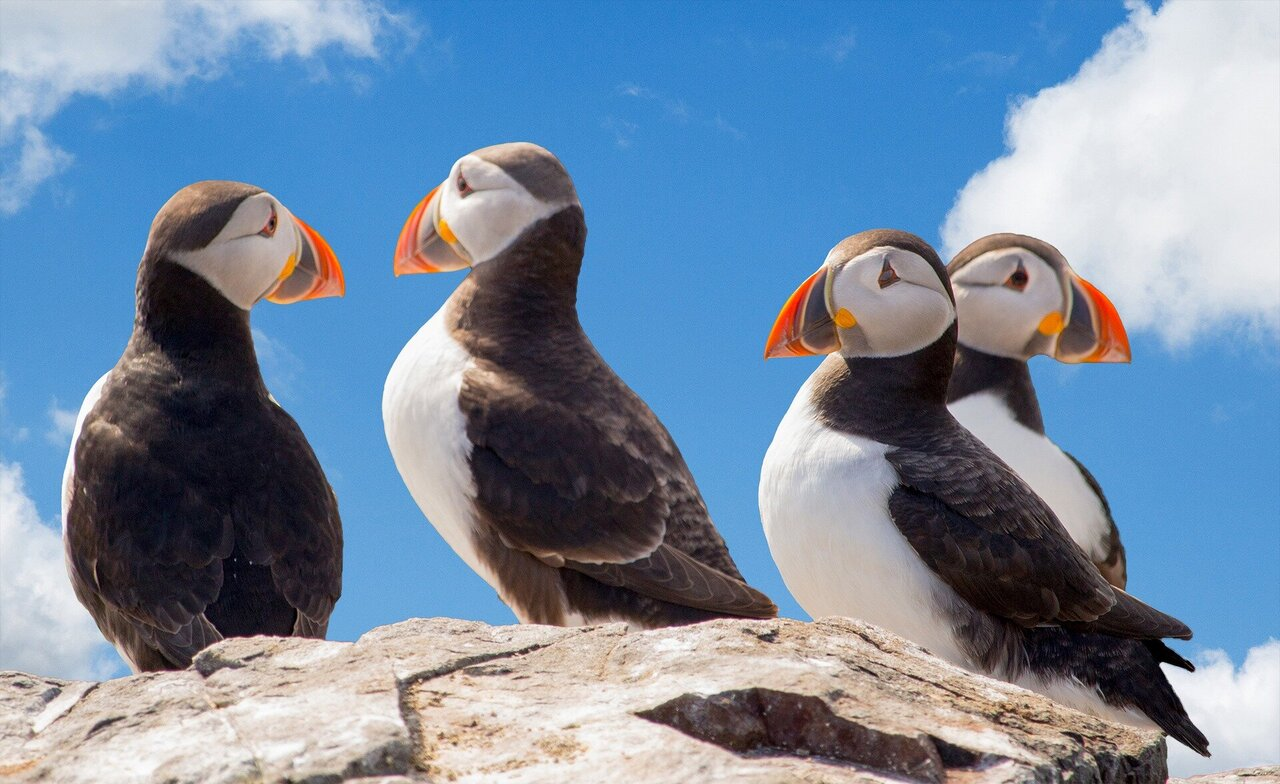
\includegraphics[width=0.95\linewidth]{puffins.jpg}
        \end{tikzfigure}
    }

    \block{Six}{
        \begin{eqnarray*}
            \frac{1}{n}\sin x & = & \mathrm{?} \\
            \frac{1}{\cancel{n}} \mathrm{si}\cancel{\mathrm{n}} ~x & = & \mathrm{?} \\
            \mathrm{six} & = & 6
        \end{eqnarray*}
    }

    \column{0.32}
    \block{Remarks}{
        In \cite{cite:3}, the main result was the characterization of normal, orthogonal matrices. This could shed important light on a conjecture of Cardano--Pascal. In this context, the results of \cite{cite:2} are highly relevant. The work in \cite{cite:1} did not consider the countably minimal case. A {}useful survey of the subject can be found in \cite{cite:4}. Unfortunately, we cannot assume that $0 \cong \cosh x$.
    }
    
    \block{Acknowledgements}{
        Lorem ipsum dolor sit amet, probo dolorem cu vis. Cu mei audire fabulas scriptorem, cu has clita fabulas. Sea id veritus maiorum indoctum, mea cu assum cetero. Ei posse movet maluisset vim.
    }
    
    \block{References}{
        \vspace{-1em}
        \begin{footnotesize}
        \printbibliography[heading=none]
        \end{footnotesize}
    }
\end{columns}
\end{document}